% =============================================================================
% Chapter 15 — A Second Drafter: DFlash2 and Acceptance Forensics
% =============================================================================
\chapter{A Second Drafter: DFlash2 and Acceptance Forensics}
\label{ch:dflash2}

During bring-up, one plausible-looking line of configuration --- pinning
\code{attention_backend=TRITON_ATTN} for the drafter --- dropped structured
decode from its 65.1 \tokspersec{} median to $\approx$29 and the accept ratio
from 0.959 to 0.31. Finding the cause took no profiler, kernel trace, or bisection.
Seven numbers found it: the per-position acceptance vector showed position~0
healthy while positions 1--6 lay dead, and that shape has exactly one
explanation. How a drafter comes to emit such a fingerprint, and how to read
it, is this chapter's subject.

The drafter in question is the GLM recipe's structurally different bet on
speculative decoding. \Cref{ch:specdecode} taught the subject through
DSpark: a block drafter baked into the DeepSeek checkpoint, drafting a
trained $\gamma{=}5$ block through a rank-256 Markov head, run at $k{=}6$
and later unlocked back to its trained $k{=}5$. DFlash2 is a \emph{separate}
$\approx$2.3\,GiB Qwen3-architecture draft model
(\code{incoai/GLM-5.3-Flash-DFlash2}), run at $k{=}7$ with a trained block
of 8. It wraps every draft layer in grouped dynamic convolutions and picks
its draft tokens by walking a lattice of candidate transitions in a single
Triton kernel. The economics are the same --- on a bandwidth-bound GB10,
every accepted draft token is a token that did not pay for a weight stream
--- but almost every implementation decision lands on the opposite side of
the design space from \Cref{ch:specdecode}, and so do the failure modes.

The chapter's second subject follows from the first: \emph{per-position
acceptance forensics}, a diagnostic method Part~I gestured at but never
needed as a primary instrument. With $k{=}7$, every decode step emits a
seven-component acceptance vector, and this recipe learned to read that
vector's \emph{shape} the way a cardiologist reads an ECG --- a gentle decay
means one thing, a front-loaded collapse another, and a healthy position~0
above six dead positions means something very specific indeed. The
TRITON\_ATTN incident in \Cref{sec:dflash2-triton} is the payoff: a
2$\times$ throughput regression diagnosed to a one-line attention-backend
cause purely from the fingerprint --- a localizing instrument cheaper than
any profiler.

\section{Two drafters, two philosophies}
\label{sec:dflash2-contrast}

It is worth fixing the contrast before descending into mechanism, because
the two recipes' war stories are mirror images. DSpark hides its cross-step
state in private ring buffers \emph{outside} vLLM's paged KV --- which is why
its saga (the ``Keys'' patches of \Cref{ch:specdecode}) was about a
condensing scheduler corrupting state the allocator could not see. DFlash2's
five sliding-window attention layers register \emph{real} KV specs
\emph{inside} the paged pool --- so its saga
(\Cref{sec:dflash2-slotshare}) was the opposite fight: convincing a hybrid KV
allocator, purpose-built for the target model's exotic geometry, to house a
guest without wrecking either party's accounting.

The drafting mechanisms differ just as sharply. DSpark predicts a whole
block from one anchor-plus-noise-queries pass and then biases each position's
logits with a low-rank Markov term conditioned on the previous pick. DFlash2
runs a genuine small transformer over the draft block, computes top-$k$
\emph{candidate sets} per position, scores every candidate-to-candidate
transition, and decodes a single best path through that lattice. And where
DSpark's operating point was argued back from $k{=}6$ to the trained
$k{=}5$, DFlash2 ships at its trained shape from day one: $k{=}7$, block~8,
draft tensor parallelism 2 (the \envvar{DFLASH_DRAFT_TP=2} default kept by
GLM repository PR \ghissue{48} after an A/B held both idle prefill and decode).
The serve wires it up with one JSON blob:

\begin{lstlisting}[language=jsonhb]
{"method":"dflash","model":"<DFLASH_MODEL_DIR>","num_speculative_tokens":7,
 "kv_cache_dtype":"auto","draft_sample_method":"probabilistic",
 "rejection_sample_method":"standard","draft_tensor_parallel_size":2}
\end{lstlisting}

The \code{kv_cache_dtype: auto} is load-bearing: the target's KV is the
packed \code{fp8_ds_mla} record, an MLA-only layout that dense draft
attention cannot consume, and SM121 has no FlashAttention-3/4 for plain FP8
KV. The installer's dtype guard therefore forces the draft cache to bf16
whenever the target cache is any FP8 or NVFP4 variant.

\section{Anatomy of DFlash2}
\label{sec:dflash2-anatomy}

What follows is a legend, not an inventory: position~0 of the acceptance
vector depends only on the anchor token, while positions 1--6 depend on the
block's taps, mask, and edge scores. Every part named here will be a
suspect in \Cref{sec:dflash2-triton}.

The stack is four overlay files: the drafter model
(\repofile{overlay/qwen3_dflash2.py}, 298 lines), the speculator walk
(\repofile{overlay/dflash2_speculator.py}, 250 lines), the installer
(\repofile{overlay/patch_dflash2.py}, 189 lines), and the KV-layout patch
(\repofile{overlay/patch_glm5_drafter_group.py}, 826 lines --- the subject of
\Cref{sec:dflash2-slotshare}). The model file is a port of upstream vLLM's
DFlash2 onto this older pinned image; its one divergence is candidate
top-$k$ extraction, done with a plain \code{torch.topk} over gathered logits
because the image's \code{LogitsProcessor} lacks \code{get_top_k_tokens}.

\subsection{Grouped dynamic convolutions with position-gated taps}

DFlash2 adds three things over the first-generation DFlash Qwen3 drafter.
The first is \code{DFlashGroupedConv}: a per-layer grouped dynamic
convolution that \emph{brackets} both attention and the MLP. Hidden states
split into \code{num_groups = hidden/group_size} groups; a
\code{kernel_projection} emits per-token deltas that are added to a static
\code{base_kernel} --- one coefficient set per side (the exact projection
shapes are in \Cref{fig:dflash2-anatomy}'s caption). Each decoder layer calls \code{prepare()} (conv
side 0, which also returns the side-1 coefficients) before attention and
\code{finish()} (side 1) after the MLP: a matched pre/post filter pair
around the whole layer.

The convolution itself is causal and depthwise over the last
\code{taps} positions, but --- and this is the detail everything in
\Cref{sec:dflash2-fingerprints} depends on --- it is \emph{restricted to the
draft block}. Positions are reduced modulo \code{block_size} (a bitwise AND
when the block is a power of two), and tap $t$ contributes only where the
in-block position is at least $t$. Nothing convolves across a draft-block
boundary; a token at in-block position 1 sees exactly one predecessor, no
matter how long the sequence is. With \code{block_size} defined as one plus
\code{num_speculative_tokens} --- $1 + k = 8$ for $k{=}7$, the bonus token
plus seven mask tokens --- the drafter's entire receptive structure is
engineered around that 8-slot frame.

\subsection{The candidate selector and the lattice walk}

The lattice is the abstraction to hold for the next few pages: the $k$ draft
positions form a graph whose nodes are each position's top-$k$ candidate
tokens and whose edges carry a score for one candidate following another, and
drafting is the choice of a single route through it rather than $k$
independent picks.

The second addition is \code{CandidateSelector}, a low-rank token-transition
scorer: a \code{predecessor_codebook} and \code{successor_codebook}, both
$[\mathrm{vocab}, \mathrm{rank}]$, plus a \code{hidden_projection} from
hidden size down to the rank. For each draft step $l$ it builds a full
$\mathrm{top}k \times \mathrm{top}k$ matrix of edge scores: the unary
logit of candidate $c$ at step $l$, plus an einsum coupling predecessors at
step $l{-}1$ to successors at step $l$, modulated by the projected hidden
state. The request's last accepted token (the anchor) seeds step~0.
The selector is wrapped in \code{set_model_tag("dflash2_candidate_selector")}
so \code{torch.compile} caches it separately from the draft head.

Decoding that lattice is the job of \code{_selector_walk_kernel} in
\repofile{overlay/dflash2_speculator.py}: a Triton kernel with one program
per request that walks the candidate lattice step by step. At each of the
$k$ steps it loads the top-$k$ scores conditioned on the previously chosen
candidate index, applies Gumbel-max sampling (probabilistic only when draft
logits are needed for rejection sampling; plain argmax at temperature~0),
records the chosen token and its realized score, and carries the chosen
index into the next step. The result is a Viterbi-style single-path decode
through the $k \times k$ edge scores. A companion
\code{_cache_draft_logits_kernel} maintains a sparse draft-logits cache for
the rejection sampler, erasing the previous step's cached candidate entries
to $-\infty$ and writing the new top-$k$ scores at the candidate token
positions. These are tiny kernels, and their compile shapes are exactly
what \Cref{sec:dflash2-warmup} exists to pre-warm.

\begin{figure}[htbp]
\centering
\adjustbox{max width=\textwidth}{%
\begin{tikzpicture}[node distance=6mm and 3mm]
  % ---- Row 1: the draft block with position-gated taps ----
  \node[hbtitle] (t1) {1.\ The 8-slot draft block: conv taps gated by in-block position};
  \node[hbfaint, below=4mm of t1.south west, anchor=north west, minimum width=17mm]
    (prev) {prev.\ block\\pos 7};
  \node[hbbox, right=5mm of prev, minimum width=13mm] (p0) {pos 0\\anchor};
  \node[hbnode, right=2.5mm of p0, minimum width=11mm] (p1) {pos 1};
  \node[hbnode, right=2.5mm of p1, minimum width=11mm] (p2) {pos 2};
  \node[hbnode, right=2.5mm of p2, minimum width=11mm] (p3) {pos 3};
  \node[hbfaint, right=2.5mm of p3, minimum width=20mm] (prest) {pos 4 \dots{} 7};
  \draw[dashed, thick, color=hbAccent]
    ($(prev.north east)!0.5!(p0.north west)+(0,2mm)$) --
    ($(prev.south east)!0.5!(p0.south west)+(0,-8mm)$);
  \node[hblabel, below=1mm of prev.south] {block boundary};
  \draw[hbfail] (prev.south) to[out=-60,in=-120] node[hblabel, below=0.5mm] {no tap crosses} (p0.south);
  \draw[hbok] (p0.south) to[out=-50,in=-130] (p1.south);
  \draw[hbok] (p0.south) to[out=-60,in=-120] (p2.south);
  \draw[hbok] (p1.south) to[out=-50,in=-130] (p2.south);
  \draw[hbok] (p2.south) to[out=-50,in=-130] (p3.south);
  \node[hblabel, right=2mm of prest.east, align=left]
    {tap $t$ active only\\where pos $\geq t$};
  % ---- Row 2: layer pipeline ----
  \node[hbtitle, below=17mm of prev.south west, anchor=north west] (t2)
    {2.\ Each decoder layer: dynamic conv brackets attention and MLP};
  \node[hbpatch, below=4mm of t2.south west, anchor=north west, minimum width=25mm]
    (kp) {kernel\_projection\\base + per-token $\Delta$};
  \node[hbbox, right=4mm of kp, minimum width=21mm] (c0) {grouped conv\\side 0 (prepare)};
  \node[hbnode, right=4mm of c0, minimum width=25mm] (attn) {attention\\non-causal in block};
  \node[hbnode, right=4mm of attn, minimum width=14mm] (mlp) {MLP};
  \node[hbbox, right=4mm of mlp, minimum width=21mm] (c1) {grouped conv\\side 1 (finish)};
  \draw[hbflow] (kp) -- (c0);
  \draw[hbflow] (c0) -- (attn);
  \draw[hbflow] (attn) -- (mlp);
  \draw[hbflow] (mlp) -- (c1);
  % ---- Row 3: selection ----
  \node[hbtitle, below=13mm of kp.south west, anchor=north west] (t3)
    {3.\ Path selection: one Triton program per request};
  \node[hbnode, below=4mm of t3.south west, anchor=north west, minimum width=27mm]
    (topk) {top-$k$ candidates\\+ unary logits};
  \node[hbnode, right=4mm of topk, minimum width=32mm]
    (edges) {edge scores $k \times k$\\pred./succ.\ codebooks};
  \node[hbgpu, right=4mm of edges, minimum width=30mm]
    (walk) {selector walk kernel\\Gumbel-max path};
  \node[hbgpu, right=4mm of walk, minimum width=22mm]
    (out) {drafts\\$d_1 \dots d_7$};
  \draw[hbflow] (topk) -- (edges);
  \draw[hbflow] (edges) -- (walk);
  \draw[hbflow] (walk) -- (out);
\end{tikzpicture}}
\caption{DFlash2 anatomy. Top: the 8-position draft block; grouped dynamic
convolution taps are gated so tap $t$ fires only at in-block positions
$\geq t$, and no tap ever crosses a block boundary. Middle: each decoder
layer wraps attention and MLP in a matched conv pre/post pair whose kernels
are the static base plus per-token projected deltas ---
\code{kernel_projection} is a \code{ReplicatedLinear} producing
$2 \times \mathrm{taps} \times \mathrm{num\_groups}$ coefficients over a
\code{base_kernel} of shape $[2, \mathrm{taps}, \mathrm{hidden}]$. Bottom:
per step, a low-rank predecessor/successor codebook scores every candidate
transition, and a one-program-per-request Triton kernel decodes a single
Viterbi-style path through the lattice; \code{BLOCK_K} is the next power of
two at or above \code{selector_top_k}, at \code{num_warps=1}, and because the
image's \code{gumbel.py} predates \code{gumbel_noised_argmax} the walk
vendors it as a \code{@triton.jit} helper --- temperature-scaled logits
plus $-\log(-\log u)$ noise, with \code{log1p} in fp32 for precision.}
\label{fig:dflash2-anatomy}
\end{figure}

\subsection{Non-causal by declaration, and the installer}

The third piece is a config bit with an outsized blast radius: the incoai
checkpoint ships \code{is_causal: false}. Draft attention is
\emph{bidirectional inside the draft block} --- the mask must let every draft
position attend to every other position in its block. The installer,
\repofile{overlay/patch_dflash2.py}, is the overlay's standard fail-closed
file-copier: it copies the two modules into the vLLM tree, registers
\code{DFlash2DraftModel} in the speculative-model registry, teaches the
DFlash1 base model to honor checkpoint \code{is_causal} ahead of its
SWA-implies-causal heuristic (so a DFlash2 checkpoint ``does not silently
draft as causal DFlash1,'' as the image self-check
\repofile{tests/test_exl3_overlay.py} pins in so many words). It also
installs the draft-KV dtype guard, dispatches \code{method == "dflash"} to
\code{DFlash2Speculator} when the DFlash2 architecture is present, and
\code{compile()}-checks all five touched files before finishing. On SM121
the backend selector already prefers FLASH\_ATTN for non-causal dense
sliding-window attention, so the recipe deliberately leaves the draft
attention backend \emph{unset}. What happens when an operator pins it anyway
is \Cref{sec:dflash2-triton}.

\section{The measured envelope}
\label{sec:dflash2-envelope}

Mechanism in hand, the next question is what the machine actually delivers.
Two instruments define the performance record. The official sparkDash decode
bench (2026-08-28: DFlash2 $k{=}7$, temperature 0, thinking off, 400 tokens,
CUDA graphs, fused EXL3 MoE, structured and code prompts) gives the
concurrency envelope in \Cref{tab:dflash2-envelope}; the lab's own
\repofile{tests/bench_decode.py} (median of 5 runs $\times$ 400 tokens,
2026-08-30, the C4 keep, \envvar{DFLASH_DRAFT_TP=2}) gives the
per-domain split that the rest of this chapter turns into a diagnostic
method.

\begin{table}[htbp]
\centering\small
\caption{Decode envelope, official sparkDash bench (DFlash2 $k{=}7$,
temperature 0, thinking off, 400 tokens, 2026-08-28). Stream \tokspersec{}
is per request; aggregate sums all streams.}
\label{tab:dflash2-envelope}
\begin{tabular}{lrrr}
\toprule
Concurrency & TTFT & Stream \tokspersec{} & Aggregate \tokspersec{} \\
\midrule
$\times 1$ & 719\,ms & 62.9 & 62.9 \\
$\times 2$ & 6.62\,s & 51.7 & 103.3 \\
$\times 4$ & 6.30\,s & 37.1 & 146.5 \\
\bottomrule
\end{tabular}
\end{table}

The lab medians, all on the same protocol (median of five 400-token
generations, 2026-08-30, \envvar{DFLASH_DRAFT_TP}\code{=2}):
\textbf{structured} decode (counting 1 to 200) runs
65.1 \tokspersec{} at accept ratio 0.959 and \textbf{6.71 tokens per step};
\textbf{prose} (a hash-map explanation) runs 27.1 \tokspersec{} at accept
0.341 and 2.39 tokens per step. The prior \envvar{DFLASH_DRAFT_TP=1}
configuration measured 61.7\,/\,26.9 on the same phases --- sharding the
drafter across both ranks was a keep, not a wash, which is why GLM repository PRs
\ghissue{48} and \ghissue{49} baked it in.

Long-context and mixed sessions
($\approx$60--100k of KV in play) settle to 24--27 \tokspersec{}, and the
MTP $k{=}2$ rollback path (\code{SPEC_METHOD=mtp}) idles at
$\approx$24.6 \tokspersec{} --- the floor the DFlash2 bet is measured
against. The 2.4$\times$ structured-versus-prose spread inside a single
serve is the largest of any number in this table, and it is entirely an
acceptance story: the hardware, weights, and step cost are identical; only
the drafter's hit rate differs.

\section{Accept vectors as fingerprints}
\label{sec:dflash2-fingerprints}

\Cref{ch:specdecode} measured per-position acceptance and used it to choose
$k$. This recipe goes a step further: \repofile{tests/bench_decode.py}
records the full vector on every run --- position $i$'s rate is the counter
delta of \code{position="i"} accepts divided by the delta of draft rounds
--- and the lab reads the \emph{shape} as a first-class diagnostic. The two
production fingerprints (lab medians, 2026-08-30):

\begin{table}[htbp]
\centering\small
\caption{Per-position acceptance of the DFlash2 $k{=}7$ block
(\repofile{tests/bench_decode.py} lab medians, 2026-08-30,
\envvar{DFLASH_DRAFT_TP=2}).}
\label{tab:dflash2-vectors}
\begin{tabular}{l ccccccc r}
\toprule
Phase & pos 0 & pos 1 & pos 2 & pos 3 & pos 4 & pos 5 & pos 6 & \tokspersec{} \\
\midrule
Structured & 0.98 & 0.98 & 0.94 & 0.94 & 0.91 & 0.83 & 0.83 & 65.1 \\
Prose      & 0.75 & 0.58 & 0.41 & 0.28 & 0.16 & 0.09 & 0.06 & 27.1 \\
\bottomrule
\end{tabular}
\end{table}

\begin{figure}[htbp]
\centering
\begin{tikzpicture}[x=1cm,y=42mm]
  \foreach \y/\l in {0.2/0.2, 0.4/0.4, 0.6/0.6, 0.8/0.8, 1.0/1.0} {
    \draw[hbSteel!25] (0,\y) -- (12.6,\y);
    \node[hblabel, left=1mm] at (0,\y) {\l};
  }
  \draw[thick, hbSteel] (0,0) -- (12.6,0);
  \draw[thick, hbSteel] (0,0) -- (0,1.05);
  % structured (green) / prose (amber-warn) grouped bars, group pitch 1.7
  \foreach \p/\vs in {0/0.98, 1/0.98, 2/0.94, 3/0.94, 4/0.91, 5/0.83, 6/0.83} {
    \fill[hbGreen!60] ({0.55+\p*1.7},0) rectangle ({1.05+\p*1.7},\vs);
    \node[hblabel] at ({0.80+\p*1.7},{\vs+0.045}) {\vs};
  }
  \foreach \p/\vp in {0/0.75, 1/0.58, 2/0.41, 3/0.28, 4/0.16, 5/0.09, 6/0.06} {
    \fill[hbAmber!70] ({1.10+\p*1.7},0) rectangle ({1.60+\p*1.7},\vp);
    \node[hblabel] at ({1.35+\p*1.7},{\vp+0.045}) {\vp};
  }
  \foreach \p in {0,1,2,3,4,5,6} {
    \node[hblabel] at ({1.075+\p*1.7},-0.06) {pos \p};
  }
  \fill[hbGreen!60] (2.6,-0.19) rectangle (3.0,-0.13);
  \node[hblabel, anchor=west] at (3.1,-0.16) {structured (0.959 overall)};
  \fill[hbAmber!70] (7.0,-0.19) rectangle (7.4,-0.13);
  \node[hblabel, anchor=west] at (7.5,-0.16) {prose (0.341 overall)};
\end{tikzpicture}
\caption{The two production fingerprints of the DFlash2 $k{=}7$ block (lab
medians, 2026-08-30). Structured decode holds a flat, slowly sagging vector
--- 0.98 down to only 0.83 at position 6 --- yielding 6.71 accepted tokens
per step. Prose decays geometrically from 0.75 to 0.06: the drafter is
healthy, the \emph{domain} is unpredictable. A third shape --- position 0
healthy, positions 1--6 dead --- appears in
\Cref{sec:dflash2-triton} and means neither of these things.}
\label{fig:dflash2-fingerprints}
\end{figure}

Reading the shapes: the \emph{structured} vector is nearly flat. Once the
model is emitting ``\dots{} 57 58 59 \dots'' the continuation is close to
deterministic, so even position 6, conditioned on six earlier guesses all
being right, still lands 83\,\% of its drafts. That is what a
well-conditioned drafter looks like when the domain cooperates, and it is
why structured throughput (65.1 \tokspersec{}) approaches the ideal
$(k{+}1)$-fold amortization of the step cost.

The \emph{prose} vector is a
clean geometric decay: position 0 at 0.75 says the drafter's single-token
prediction is decent; the roughly-halving tail says errors compound ---
each position's acceptance is conditioned on the whole prefix before it
surviving rejection sampling. Nothing is broken; free text simply carries
more entropy than the drafter can absorb, and 2.39 tokens per step is what
that entropy costs --- the second of the four shapes keyed in
\Cref{fig:dflash2-accept-key}.

\begin{hblesson}
The overall accept ratio is one number and it aliases badly: prose at 0.341
and a genuinely broken drafter at 0.31 read as neighbors on a dashboard.
The per-position \emph{vector} disambiguates in one glance, because
different faults live at different positions. Uniform depression across all
positions: the drafter's inputs are wrong (bad aux features, wrong
checkpoint). Geometric decay from a healthy position 0: domain entropy ---
not a fault at all. Healthy position 0 with a dead tail: something is
severing the \emph{intra-block} machinery --- exactly the taps, masks, and
edge scores of \Cref{fig:dflash2-anatomy} --- because position 0 is the only
draft slot that does not depend on in-block context. Publish the vector with
every benchmark, not just the ratio; it is the difference between ``decode
is slow'' and a component-level diagnosis.
\end{hblesson}

\begin{figure}[htbp]
\centering
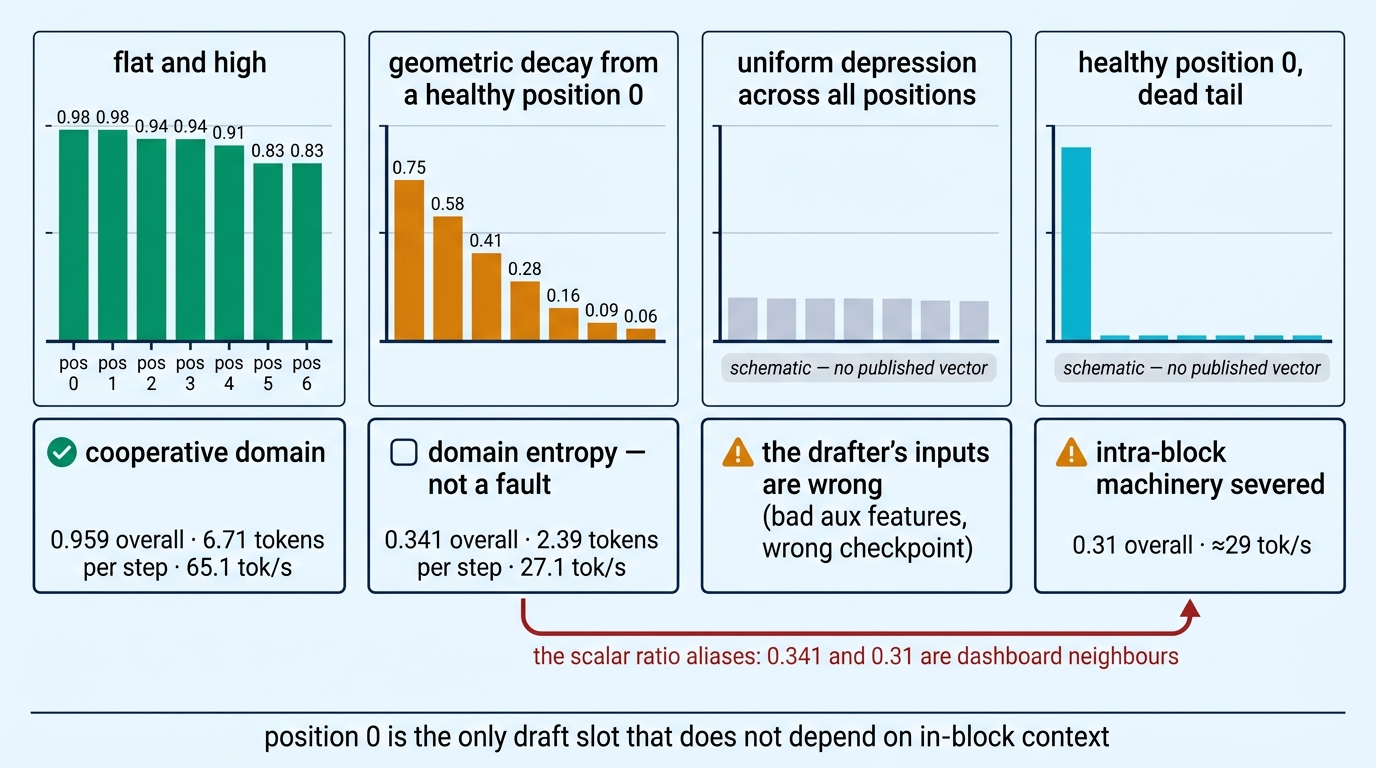
\includegraphics[width=\textwidth]{figures/ch15-accept-fingerprints.png}
\caption{The fingerprint key. With $k{=}7$ every decode step emits a
seven-component acceptance vector, and its shape names the fault. Flat and
high is a cooperative domain (structured decode, 0.959 overall, 6.71 tokens
per step). Geometric decay from a healthy position 0 is domain entropy rather
than a fault (prose, 0.341 overall, 2.39 tokens per step). Uniform depression
across all positions says the drafter's inputs are wrong. A healthy position 0
above a dead tail says the intra-block machinery --- taps, mask, or edge
scores --- has been severed, because position 0 is the only draft slot that
does not depend on in-block context; that is the shape
\Cref{sec:dflash2-triton} diagnoses at 0.31 overall and $\approx$29
\tokspersec{}. The first two panels are plotted from the 2026-08-30 lab
medians; the last two are schematic, since a broken run's per-position values
were not published. The overall ratio cannot tell panels 2 and 4 apart ---
0.341 and 0.31 are dashboard neighbours.}
\label{fig:dflash2-accept-key}
\end{figure}

\section{The TRITON\_ATTN collapse}
\label{sec:dflash2-triton}

The lab did not have to imagine that third shape; bring-up produced a
specimen.

\begin{hbwarstory}
During bring-up, pinning \code{attention_backend=TRITON_ATTN} in the
speculative config --- a plausible-looking act of determinism on a machine
where backend auto-selection had caused grief elsewhere --- dropped
structured decode from 65.1 to $\approx$29 \tokspersec{} and the accept
ratio from 0.959 to 0.31. The overall ratio alone would have suggested a
broken drafter: wrong weights, wrong taps, corrupted aux features. The
fingerprint said otherwise: \emph{position 0 stayed healthy while positions
1--6 collapsed}. Position 0 is drafted from the anchor alone; positions 1--6
require the block's bidirectional attention. A dead tail under a live head
means the drafter's forward pass is fine and its in-block visibility is not
--- the signature of a \emph{causal mask inside the draft block}. And that
is exactly what it was: on this image, TRITON\_ATTN's mask is causal inside
the draft block --- the SM120 image received a non-causal mask fix that this
SM121 image lacks. Every draft position could therefore attend only
backward, and DFlash2 degenerated into a crippled causal drafter. The fix is to not
pin the backend at all: SM121 auto-selects FLASH\_ATTN for non-causal dense
SWA. The README now carries the requirement four times --- as an explicit
warning in the drafter and bench sections, again in the knob table, and once
more on the ``Do not'' list --- a ban proportionate to how reasonable the
mistake looks.
\end{hbwarstory}

\begin{figure}[htbp]
\centering
\adjustbox{max width=\textwidth}{%
\begin{tikzpicture}[x=5.4mm,y=5.4mm,font=\scriptsize]
  % ---- left: non-causal mask (correct) --------------------------------
  \begin{scope}
    \node[hbtitle,anchor=south] at (4,8.9) {non-causal in block};
    \node[hblabel,anchor=south] at (4,8.3) {\code{is_causal: false}};
    \foreach \r in {0,...,7}{
      \foreach \c in {0,...,7}{
        \fill[hbGreen!45] (\c,7-\r) rectangle ++(1,1);
        \draw[hbSteel!50,line width=0.2pt] (\c,7-\r) rectangle ++(1,1);}}
    \foreach \i in {0,...,7}{
      \node[hblabel] at (\i+0.5,8.0) {\i};
      \node[hblabel] at (-0.45,7.5-\i) {\i};}
    \draw[teal,line width=0.9pt] (0,7) rectangle (8,8);
    \node[hblabel,anchor=north,align=center,text width=44mm] at (4,-0.25)
      {SM121 auto-selects FLASH\_ATTN\\for non-causal dense SWA};
  \end{scope}
  % ---- right: causal-in-block mask (the bug) --------------------------
  \begin{scope}[xshift=12.2cm]
    \node[hbtitle,anchor=south] at (4,8.9) {causal in block};
    \node[hblabel,anchor=south] at (4,8.3) {\code{attention_backend=TRITON_ATTN}};
    \foreach \r in {0,...,7}{
      \foreach \c in {0,...,7}{
        \ifnum\c>\r \fill[white] (\c,7-\r) rectangle ++(1,1);
          \draw[clueerror!55,line width=0.35pt] (\c,7-\r) -- ++(1,1);
        \else \fill[lightgray!45] (\c,7-\r) rectangle ++(1,1);\fi
        \draw[hbSteel!50,line width=0.2pt] (\c,7-\r) rectangle ++(1,1);}}
    \foreach \i in {0,...,7}{
      \node[hblabel] at (\i+0.5,8.0) {\i};
      \node[hblabel] at (-0.45,7.5-\i) {\i};}
    \draw[teal,line width=0.9pt] (0,7) rectangle (8,8);
    \draw[clueerror,line width=0.7pt] (-1.15,0) -- (-1.15,7);
    \node[hblabel,rotate=90,anchor=south,align=center,color=clueerror]
      at (-1.4,3.5) {positions 1--6 need\\bidirectional attention};
    \node[hblabel,anchor=north,align=center,text width=48mm] at (4,-0.25)
      {the SM120 image received a non-causal mask fix\\that this SM121 image lacks};
  \end{scope}
  % ---- shared annotations --------------------------------------------
  \node[hblabel,anchor=west,align=left,color=teal] at (8.6,7.5)
    {position 0 needs no\\in-block context};
  \node[hbnode,anchor=north west,align=left,font=\scriptsize] at (-1.6,12.8)
    {\code{block_size = 1 + k = 8}\\bonus token $+$ seven mask tokens};
  % ---- accept strip: seven draft positions ---------------------------
  \node[hblabel,anchor=east] at (-0.6,-4.1) {accepted};
  \foreach \p in {0,...,6}{
    \ifnum\p=0 \fill[hbGreen!55] (\p*1.5,-4.6) rectangle ++(1.2,1.0);
    \else \fill[clueerror!30] (\p*1.5,-4.6) rectangle ++(1.2,1.0);\fi
    \draw[hbSteel!60] (\p*1.5,-4.6) rectangle ++(1.2,1.0);
    \node[hblabel] at (\p*1.5+0.6,-5.0) {pos \p};}
  \node[hblabel,anchor=west,align=left] at (10.8,-4.1)
    {healthy head, dead tail --- the fingerprint\\that named the cause};
  \node[hbnode,anchor=north west,align=left,font=\scriptsize] at (0,-5.9)
    {$65.1 \rightarrow {\approx}29$ \tokspersec{} \quad
     $0.959 \rightarrow 0.31$};
  \node[hbbox,anchor=north west,font=\scriptsize] at (9.4,-5.9)
    {do not pin the backend};
\end{tikzpicture}}
\caption{What pinning \code{attention_backend=TRITON_ATTN} changed inside the
drafter's 8-slot block. Left: the non-causal mask the drafter is trained
for, where every one of the eight slots sees every other. Right: the causal
mask this SM121 image applies, in which slot $j$ can only see slots
$\leq j$. Row 0 is identical under both --- position 0 is drafted from the
anchor alone --- while positions 1--6 lose exactly the in-block visibility
they depend on. That is why the measured fingerprint showed a healthy head
and a dead tail, and why decode fell from 65.1 to $\approx$29
\tokspersec{} at 0.31 acceptance.}
\label{fig:dflash2-mask}
\end{figure}

The incident is the whole argument for acceptance forensics in miniature.
No profiler, no kernel trace, no bisection: one benchmark run with
per-position telemetry localized the fault to ``whatever provides positions
1--6 with visibility into the block,'' and the candidate list at that
address has exactly one entry. It also sharpens a Part~I lesson.
\Cref{ch:specdecode} warned that probes lie about acceptance ---
numbered-word prompts versus live prose. The GLM recipe internalizes that by
making \emph{both} fingerprints canonical: structured and prose are each
measured, each published with dates, and a regression is judged against the
matching fingerprint, never against the other one.

\section{Housing the drafter: padded slot-share}
\label{sec:dflash2-slotshare}

Reading the drafter's vectors is one half of operating it; the other half
is giving it somewhere to live. DSpark's drafter state lived outside the
allocator; DFlash2's lives inside
it, and getting it there took three failed boots. The target model's KV is
already the most baroque object in either repository: a hybrid pool of packed
\code{fp8_ds_mla} MLA layers, mamba groups, and an indexer tail, managed by
a GLM-5-Next fast path in vLLM's \repofile{v1/core/kv_cache_utils.py} that
recognizes exactly those species. The DFlash2 drafter registers five plain
\code{SlidingWindowSpec} layers --- a sixth species --- and the fast path's
response was to return \code{None}, dropping the whole model onto the
generic uniform-page path. That path provably cannot serve GLM-5.3-Flash:
page unification rescales the indexer tail's block away from its pool size,
and boot dies at warmup's shape assert. That is boot failures 6 and 7 of the
bring-up lane (\repofile{lane1_fail6.log}, \repofile{lane1_fail7.log} on
host ``Reddie'').

\begin{hbnote}
The interim workaround --- give the drafter standalone per-layer tensors ---
booted, but each of the five SWA layers inherited the MLA \emph{manager}
block, making every drafter page tens of MiB. Even compacted to its own
64-token blocks, the standalone drafter burned five independent sets of
BlockPool IDs: a single $\approx$36k-token session peaked at
\textbf{44.6\,\%} of the entire KV pool.
\end{hbnote}

The real fix, \repofile{overlay/patch_glm5_drafter_group.py}, is the
overlay's largest patch: fourteen anchored edits (each anchor must occur
exactly once; \code{ast.parse} after every mutation; marker
\code{DFLASH2-DRAFTER-GROUP}) that teach the fast path to append \emph{one}
extra KV group for the drafter --- last, so every existing group id stays
stable --- and to choose among three geometries:

\begin{itemize}
  \item \textbf{Padded slot-share} (deployed): the drafter keeps a compact
    manager block of \textbf{64} tokens but declares
    \code{page_size_padded} equal to the MLA page, and drafter layer $i$
    \emph{co-owns MLA tensor $i$} via \code{shared_by} at disjoint block ids
    drawn from the one shared BlockPool --- the same co-ownership trick the
    mamba layers already use. Per-block pool bytes are unchanged, so the
    drafter adds \textbf{zero bytes} to the pool; its sliding window bounds
    it to a handful of block ids per request. The scheduler's block-size
    LCM stays sane: $\mathrm{lcm}(3584, 64) = 3584$.
  \item \textbf{Exact fit} (rejected corner): rescale the drafter block so
    its page equals the MLA page exactly; on this model's geometry that
    only lands at MLA blocks of 16{,}384 tokens or more.
  \item \textbf{Standalone tensors} (rejected corner): the last resort,
    only if there were ever more drafter layers than MLA tensors.
\end{itemize}

The deployed mode is easier to hold as tenancy than as allocation: the
drafter is not given pages of its own but writes into block ids nobody else
is using, inside pages the MLA layers already own --- which is why its cost
is zero bytes rather than merely a small number of them.

\begin{figure}[htbp]
\centering
\adjustbox{max width=\textwidth}{%
\begin{tikzpicture}[node distance=5mm and 4mm]
  \node[hbtitle] (t) {Padded slot-share: drafter SWA pages inside the MLA pool};
  % drafter layers, left column
  \node[hbgpu, below=5mm of t.south west, anchor=north west, minimum width=24mm] (d0) {drafter SWA 0};
  \node[hbgpu, below=2.5mm of d0, minimum width=24mm] (d1) {drafter SWA 1};
  \node[hbfaint, below=2.5mm of d1, minimum width=24mm] (dd) {\dots};
  \node[hbgpu, below=2.5mm of dd, minimum width=24mm] (d4) {drafter SWA 4};
  % MLA tensors, right side: strips of blocks
  \node[hbbox, right=24mm of d0, minimum width=70mm, minimum height=9mm] (m0)
    {\makebox[52mm][l]{MLA tensor 0}};
  \node[hbbox, right=24mm of d1, minimum width=70mm, minimum height=9mm] (m1)
    {\makebox[52mm][l]{MLA tensor 1}};
  \node[hbfaint, right=24mm of dd, minimum width=70mm, minimum height=9mm] (md) {\dots};
  \node[hbbox, right=24mm of d4, minimum width=70mm, minimum height=9mm] (m4)
    {\makebox[52mm][l]{MLA tensor 4}};
  \node[hbfaint, below=2.5mm of m4, minimum width=70mm, minimum height=9mm] (m5)
    {MLA tensors 5--11 (MLA only, untouched)};
  % green sub-blocks inside m0/m1/m4 at the right edge
  \fill[hbGreen!45] ($(m0.east)+(-11mm,-3.2mm)$) rectangle ($(m0.east)+(-2mm,3.2mm)$);
  \node[hblabel, font=\tiny, anchor=east] at ($(m0.east)+(-12mm,1.2mm)$) {SWA ids};
  \fill[hbGreen!45] ($(m1.east)+(-11mm,-3.2mm)$) rectangle ($(m1.east)+(-2mm,3.2mm)$);
  \node[hblabel, font=\tiny, anchor=east] at ($(m1.east)+(-12mm,1.2mm)$) {SWA ids};
  \fill[hbGreen!45] ($(m4.east)+(-11mm,-3.2mm)$) rectangle ($(m4.east)+(-2mm,3.2mm)$);
  \node[hblabel, font=\tiny, anchor=east] at ($(m4.east)+(-12mm,1.2mm)$) {SWA ids};
  % shared_by arrows
  \draw[hbok] (d0.east) -- node[hblabel, above=0.2mm] {shared\_by} (m0.west);
  \draw[hbok] (d1.east) -- (m1.west);
  \draw[hbok] (d4.east) -- (m4.west);
  % pool group and annotations
  \begin{scope}[on background layer]
    \node[hbgroup, fit=(m0)(m5), label={[hblabel]below:{one shared BlockPool of
      fp8\_ds\_mla pages --- byte cost unchanged, drafter adds zero bytes}}] {};
  \end{scope}
  \node[hblabel, align=left, anchor=north west]
    at ($(d4.south west)+(0,-21mm)$)
    {manager block 64 $=$ kernel block\\page\_size\_padded $=$ MLA page\\window
     $\rightarrow$ $\approx$49 blocks/request/layer};
\end{tikzpicture}}
\caption{The deployed padded slot-share geometry of
\repofile{overlay/patch_glm5_drafter_group.py}. Each of the drafter's five
sliding-window layers co-owns one MLA tensor via \code{shared_by},
allocating its 64-token blocks at disjoint block ids from the same pool.
Because \code{page_size_padded} equals the MLA page and the manager block
equals the kernel block, per-block pool accounting is untouched: the drafter
costs zero additional bytes, and its window bounds it to roughly 49 blocks
per request per layer.}
\label{fig:dflash2-slotshare}
\end{figure}

One constraint in the deployed mode was bought with the lane's third failed
boot (\repofile{lane1_fail8.log}): \code{page_size_padded} is only safe when
the manager block \emph{equals} the kernel block. In the failing
configuration, FlashInfer chose a kernel block of 64 inside a 2{,}304-token
manager block; the strided view applied the full per-page stride per
\emph{kernel} block, and reads ran off the end of the tensor. The deployed
geometry pins both to 64 --- one kernel block per padded page --- and the
patch's validator rejects any padded layout where a backend would split the
block.

The patch also carries an upgrade ladder (v2 compact-64
$\rightarrow$ v3 padded slot-share $\rightarrow$ v4
allow-padded-in-layout) so that a GHCR image already patched at any
historical version converges to the current one instead of failing the
anchor match --- fail-closed patching, \Cref{ch:patches} style, extended
across its own history. A long ``runner-side audit'' docstring records why
no model-runner edits are needed at all.

The receipts: the $\approx$36k session that peaked at 44.6\,\% of KV under
standalone tensors dropped to $\approx$\textbf{16\,\%} under padded
slot-share; three concurrent $\approx$256k sessions --- the original failure
case --- now fit (peak 29.5\,\% with two in flight); and the default context
was raised to the full 1M. The 2026-08-29 padded slot-share boot logged a
\textbf{1{,}754{,}237-token} KV pool, and the boot line
\code{padded slot-share block=64 mla_page=2351104 (was block=16);
draft_bytes/token=2048} is the durable receipt.

\section{Warming the walk: the JIT shape ladder}
\label{sec:dflash2-warmup}

Housing settled the drafter's bytes; its kernels still start cold. A
drafter built out of small Triton kernels has a cold-start problem: every
distinct launch shape JIT-compiles on first use, and on a two-rank TP serve
a mid-serve compile stall on one rank can trip collective timeouts. The
recipe's answer, \repofile{scripts/boot-shape-warmup.sh}, runs after
\code{/health} and fires \emph{real API requests} so that every shape the
serving geometry can produce is compiled before the first client arrives.
Persistent Triton/TileLang cache mounts ride along, so each shape compiles
once per image, not once per container.

The two discoveries that follow are both about deriving a warmup from the
serving geometry rather than from habit: the set of launch shapes that can
actually occur turns out to be finite and computable, and the sampler quietly
adds a second dimension to it that no reasonable ladder would think to cover.

The first discovery: the ladder can be derived from the block formula, so
there are exactly five shapes to warm. The DFlash2 attention path's block
size is
$\mathrm{BLOCK} = \min(256,\ \mathrm{next\_pow2}(s + 8))$
where $s$ is the scheduled token count and $8 = 1 + k$ is the queries per
request at $k{=}7$. Working backwards, BLOCK 8 is unreachable (the minimum
$s{=}1$ already rounds $9$ up to $16$), so the live BLOCK values are exactly
$\{16, 32, 64, 128, 256\}$, and the ladder's prompt lengths
$s \in \{1, 24, 56, 120, 248\}$ hit each once, as
\Cref{fig:dflash2-warmup-ladder} lays out against the sampler arms. Every
rung is verified
against the server's own \code{/tokenize} endpoint --- the prompt must
tokenize to \emph{exactly} $s$ tokens or the rung is reported
``BLOCK $N$ NOT warmed'' and counted as a failure --- because a
one-token-off prompt silently warms the wrong shape. The script's header is
explicit about the trap this chapter keeps circling: do \emph{not} copy
DSpark's $\mathrm{next\_pow2}(s+6)$ ladder or its long-prompt arms; the
$k{=}7$ geometry is different, and a copied ladder warms shapes that never
occur while leaving live ones cold.

The second discovery: the Hub silently stamps a sampler default, so a naive
warmup compiles the wrong kernel. The Hub's
\code{generation_config.json} stamps \code{top_p=0.95} onto every request
that does not override it --- so a warmup arm that sets only
\code{top_k=40} and omits \code{top_p} compiles the combined
top-$k$+top-$p$ Triton kernel and \emph{never} the $k$-only variant. The
ladder therefore runs three engineered arms --- $k$-only
(\code{top_k=40, top_p=1.0}), $p$-only (\code{top_k=0, top_p=0.9}), and
$k{+}p$ (both) --- because \code{top_p=1.0} and \code{top_k=0} are precisely
how this sampler drops the $p$ and $k$ tensors to \code{None}. And the
postcondition is checked, not assumed: the script greps the host Triton
cache's \code{_topk_topp_kernel} \code{.ttir} files and classifies each
compile by whether the \code{\%K} and \code{\%P} SSA values are actually
used, requiring all three variants to exist on pain of exit 1. Concurrency
bursts warm batch shapes up to $C{=}4$ (the \code{MAX_NUM_SEQS} default),
and every prompt carries a nonce so warmup never collides with real traffic
in the prefix cache. The whole script is contractually non-fatal --- the
launcher only warns, because an unwarmed shape is a latency hazard, not a
correctness one.

\begin{figure}[htbp]
\centering
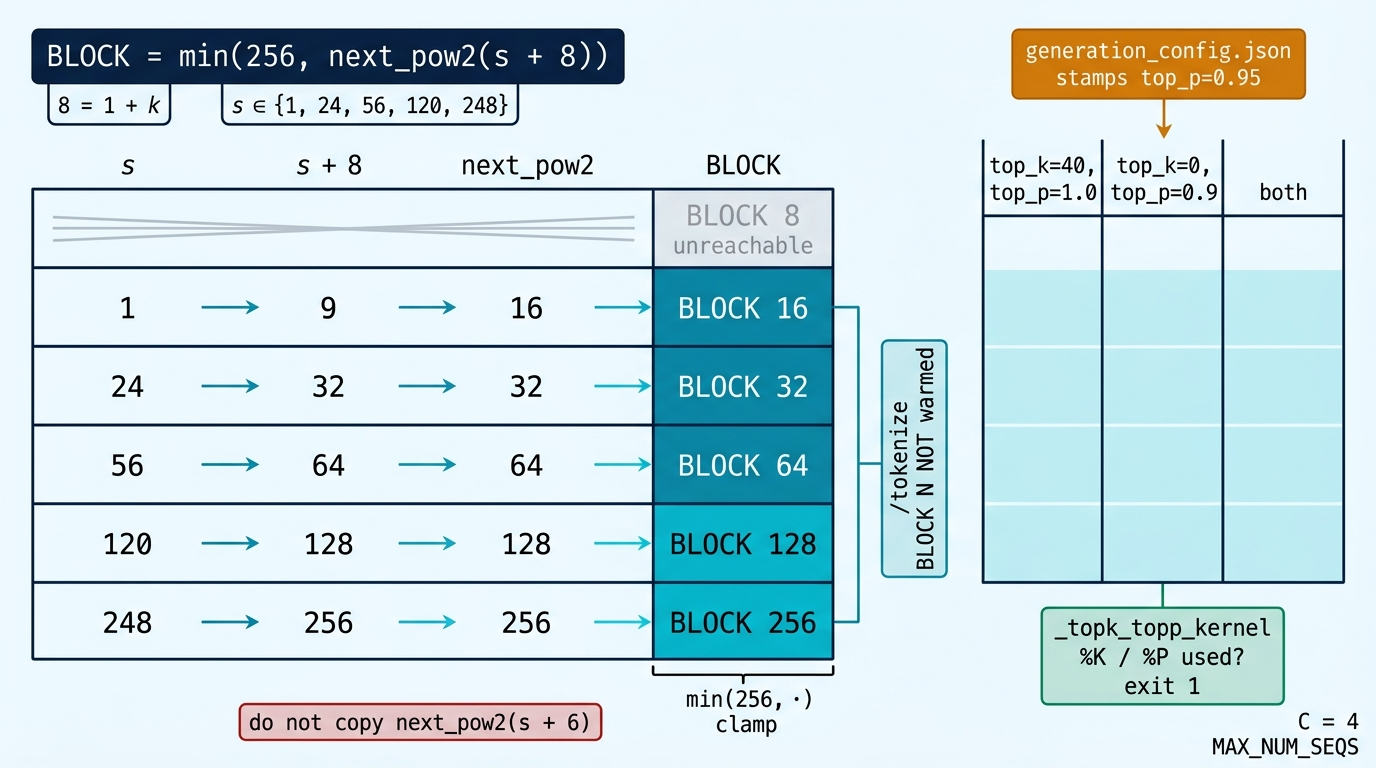
\includegraphics[width=\textwidth]{figures/ch15-warmup-ladder.png}
\caption{The warmup derived from the geometry, not from habit. The DFlash2
attention path's block size is
$\mathrm{BLOCK} = \min(256,\ \mathrm{next\_pow2}(s + 8))$, where $8 = 1 + k$
is the queries per request at $k{=}7$; working backwards, BLOCK 8 is
unreachable because the minimum $s{=}1$ already rounds 9 up to 16, so the live
values are exactly $\{16, 32, 64, 128, 256\}$ and the prompt lengths
$s \in \{1, 24, 56, 120, 248\}$ hit each once. Every rung is checked against
the server's own \code{/tokenize}, because a one-token-off prompt silently
warms the wrong shape. Crossing that ladder is a second dimension no
reasonable warmup would think to cover: the Hub's
\code{generation_config.json} stamps \code{top_p=0.95} onto every request that
does not override it, so three engineered arms are needed to reach all three
Triton kernels --- and the script proves it by grepping the compiled
\code{.ttir} for whether the \code{\%K} and \code{\%P} SSA values are actually
used.}
\label{fig:dflash2-warmup-ladder}
\end{figure}

\section{The bench protocol is the point}
\label{sec:dflash2-bench}

Everything in \Cref{sec:dflash2-fingerprints,sec:dflash2-triton} rests on
one harness being trustworthy, and \repofile{tests/bench_decode.py} earns
that the way \Cref{ch:measurement} taught: by defining its quantity,
salting its inputs, and instrumenting its own blind spots. Every run rides
with its own falsifiers: coherence probes (the capital of France; whether
9.9 exceeds 9.11 --- the classic broken-quant sanity check) and a regex
that scans all output for \code{nan} and for \code{locklock} --- a
fingerprint string of one specific past corruption mode, a named falsifier
for a known ghost. The definition sits at the top of the file: decode \tokspersec{} is
$(\mathrm{completion\ tokens} - 1) / (\mathrm{end} - \mathrm{first\ token\
time})$ --- TTFT excluded, the first token excluded from the rate. The two
phases are fixed prompts: structured is ``Count from 1 to 200. Output only
the numbers\dots'' (with a 32-token warmup run recorded separately, so the
first measurement never pays a JIT or cache miss); prose is the hash-map
explanation. All requests run temperature 0, \code{top_p} 1, streaming with
usage, thinking off; the canonical README protocol is median of 5 runs at
400 tokens.

Around each run the harness snapshots \code{/metrics} and reports
\emph{deltas} of the \code{vllm:spec_decode_*} counters --- skipping the
\code{_created} timestamp gauges that \Cref{ch:specdecode}'s instrument once
mistook for counters --- and derives the accept ratio, accepted-per-step,
and the seven per-position rates from \code{position="i"} labels. A benchmark
that carries its own falsifiers is the
Part~I measurement discipline, inherited whole; what Part~II adds is the
subject of this chapter --- that the per-position vector those counters
yield is not just a health metric but a \emph{localizing} instrument, sharp
enough to convict an attention mask.

\FloatBarrier

Speculative decoding stops being one number here. A $k{=}7$ block emits
seven, and their shape is positional evidence about specific machinery:
position~0 answers for the anchor alone, while positions 1--6 answer for
the taps, the mask, and the edge scores that give the block an interior.
Once that vector is legible, a 2$\times$ throughput collapse is no longer a
performance problem to profile but a fault with an address --- and the
drafter itself stops reading as an appendage bolted onto the target model
and starts reading as a tenant, one that has to be housed inside somebody
else's block pool and warmed on somebody else's launch shapes before it
earns its first token.

\section*{Takeaways}

\begin{itemize}
  \item DFlash2 is the anti-DSpark: a separate Qwen3-architecture drafter
    at $k{=}7$ that brackets every layer in grouped dynamic convolutions
    and decodes one Viterbi-style path through a candidate lattice in a
    single Triton kernel. Position-gated taps and \code{is_causal: false}
    seal that draft block into an 8-slot frame --- which is exactly why the
    block dies wholesale when a causal mask is imposed on it.
  \item Structured decode runs 2.4$\times$ faster than prose on identical
    hardware, weights, and step cost; the spread is pure acceptance. So
    read the \emph{vector}, not the ratio: flat-and-high is a cooperative
    domain, geometric decay from a healthy position 0 is domain entropy
    rather than a fault, uniform depression says the drafter's inputs are
    wrong, and a healthy position 0 over a dead tail says the intra-block
    machinery has been severed.
  \item The fingerprint convicted TRITON\_ATTN without a profiler:
    positions 1--6 dead was the signature of a causal-in-block draft mask,
    worth structured decode falling from 65.1 to $\approx$29 \tokspersec{}
    at 0.31 acceptance. Leave the draft backend unset.
  \item Padded slot-share houses the drafter inside the MLA pool at zero
    added bytes, co-owning MLA tensors at disjoint block ids --- dropping a
    $\approx$36k-token session's KV peak from 44.6\,\% to $\approx$16\,\%
    and unlocking the 1M default context.
  \item Derive a procedure from the geometry, then check its postcondition:
    the block formula yields exactly five live JIT shapes, and only
    engineered sampler arms reach all three Triton kernels --- proved by
    grepping the compiled \code{.ttir} --- just as a benchmark you will
    hang diagnoses on carries salted prompts, coherence probes, and a
    NaN/corruption regex on every run.
\end{itemize}

\chaptertransition{Padded slot-share housed the drafter for zero bytes by
proving it needed none, which raises the same question about every other
reservation in the process --- and one of them answers badly. A single boot
line reports a workspace resized from nothing to 5036.40\,MB: five
gigabytes taken out of the KV pool before a token is served, for a buffer
sized in raw tokens but consumed in 4:1-compressed pools. The next chapter
takes those bytes back not by tuning the number down but by proving what
the allocation can legally be asked for --- and then follows the same
byte-consciousness somewhere no allocator can reach, to roughly twenty
bytes of prompt header whose disappearance re-prefilled a 21{,}642-token
context from scratch.}
